\documentclass[a4paper, 12pt]{article}
\usepackage[total={17cm,25cm}, top=2.5cm, left=2.5cm, right=2.5cm,  includefoot]{geometry}
\usepackage[utf8]{inputenc}
\usepackage{array}
\usepackage{multirow}
\usepackage{hhline}
\usepackage{gensymb}
\usepackage{graphicx}
\graphicspath{ {} }
\usepackage[czech]{babel}
\usepackage{enumitem}
\usepackage{pdfpages}
\usepackage{amsmath}
\usepackage{verbatim}
\usepackage{listings}
\usepackage{hyperref}
\usepackage{amssymb}


\pagestyle{empty} % vypne číslování stránek




\usepackage[OT2,OT1]{fontenc}
\newcommand\cyr
{
\renewcommand\rmdefault{wncyr}
\renewcommand\sfdefault{wncyss}
\renewcommand\encodingdefault{OT2}
\normalfont
\selectfont
}
\DeclareTextFontCommand{\textcyr}{\cyr}
\def\cprime{\char"7E }
\def\cdprime{\char"7F }
\def\eoborotnoye{\char’013}
\def\Eoborotnoye{\char’003}


\begin{document}



\begin{titlepage}
\begin{center}
\noindent
\Large \textbf{České vysoké učení technické v Praze }\\ Fakulta stavební
\vspace{5cm}

\huge

%vložení loga cvut
\begin{figure}[h!]
	\centering
	
\includegraphics[width=7cm]{pictures/logo.png}
\end{figure}

\vspace{0.5cm}

Algoritmy v digitální kartografii \\

\vspace{3cm}

\Huge  
Digitální model terénu a jeho analýzy\\

\vspace{2cm}

\Large
Bc. Petra Pasovská \\
Bc. David Zahradník \\

\end{center}

\end{titlepage}




\pagestyle{plain}     % zapne obyčejné číslování
\setcounter{page}{1}  % nastaví čítač stránek znovu od jedné

\tableofcontents
\newpage

\section{Zadání}
Níže uvedené zadání je kopie ze stránek předmětu. 

\begin{figure}[h!]
	\centering
	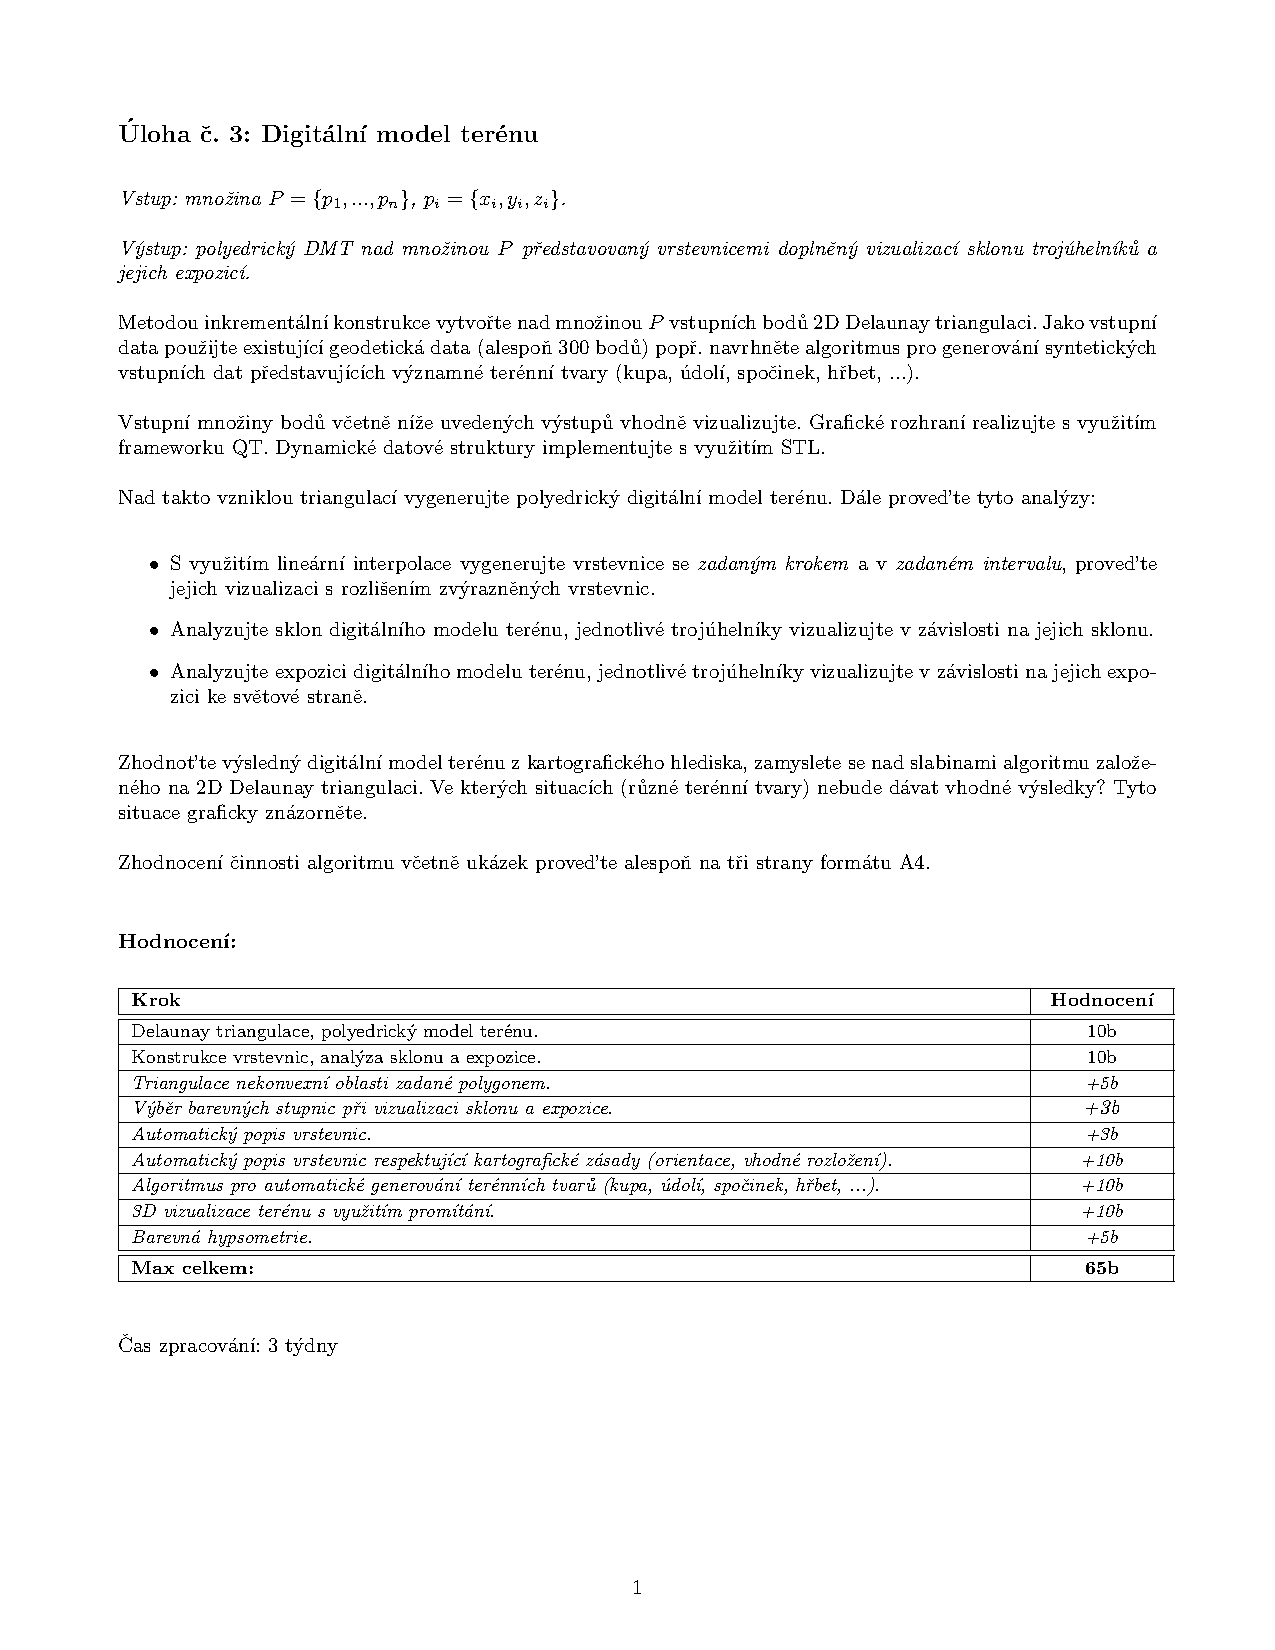
\includegraphics[width=17cm]{zadani.pdf}
\end{figure}

\subsection{Údaje o bonusových úlohách}
V rámci bonusových úloh byl vytvořen výběr barevných stupnic pro vizualizaci sklonu a expozice. Dále jsou v rámci aplikace generované některé terénní tvary.



\section{Popis a rozbor problému}
Hlavním cílem této úlohy je tvorba aplikace, která nad výškopisnými body vytvoří  triangulaci, vrstevnice a vypočte sklon a expozici k světovým stranám.\\
\\
Obecně triangulační algoritmy jsou nejvíce zkoumané algoritmy digitální kartografie v dnešní době. Slouží k různým účelům např. tvorba digitálního modelu terénu, plánování pohybu robotů, detekce otisků prstů.  [Zdroj: 1]\\
\\
Při triangulaci je kladen důraz na to, aby vytvořené trojúhelníky byly pokud možno rovnostranné. V případě, že takovéto trojúhelníky sestavíme, každý z vytvořených trojúhelníků musí co nejlépe reprezentovat hodnotu povrchu. Zároveň je nutné, aby byla produkována jednoznačná triangulace nezávisle na počátečním bodě či na orientaci množiny bodů.  triangulace tyto podmínky obecně splňuje, přesto existují výjimky, kdy nemá Delaunay triangulace jednoznačné řešení. Tento stav může nastat pro určité množiny dat, např. pravoúhlý grid. [Zdroj: 2]\\
\\
Delaunay triangulace je velmi podobná Dirichletově teselaci, která rozdělí body unikátní množinou polygonů, které jsou označovány jako Thiessenovy polygony či Voronoiovy diagramy. Voronoiovy diagramy jsou takové polygony, které vytvoří kolem všech bodů takové oblasti, že všechna místa uvnitř leží nejblíže k danému bodu. \\
\\
Voronoiovy diagramy mají v dnešní době řadu využití. V meteorologii se využívají pro určení množství srážek v daném území, v astronomii pro studium galaxií, v molekulární biologii pro hledání tunelů v molekulách, v geografii pro sledování osídlení či pro plánování cest při pohybu robotů. Voroniovy diagramy se vyskytují i v přírodě, můžeme je nalézt na kůži žirafy, na krunýři želvy, na povrchu pouště Atacamy či na křídle vážky. [Zdroj: 3]

\begin{figure}[h!]
\centering
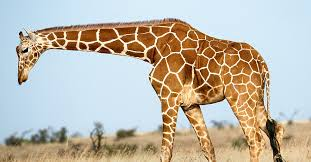
\includegraphics[width=5cm]{pictures/zirafa.jpg}
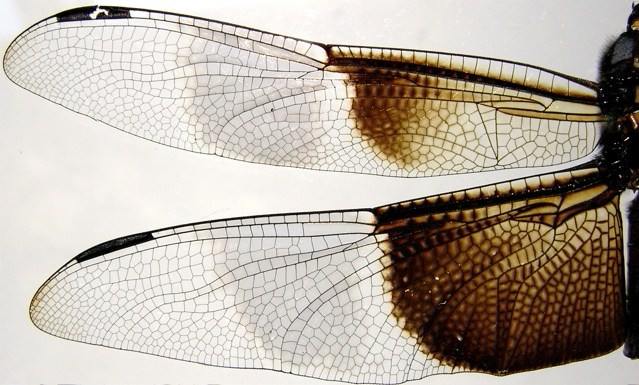
\includegraphics[width=5cm]{pictures/vazka.jpg}
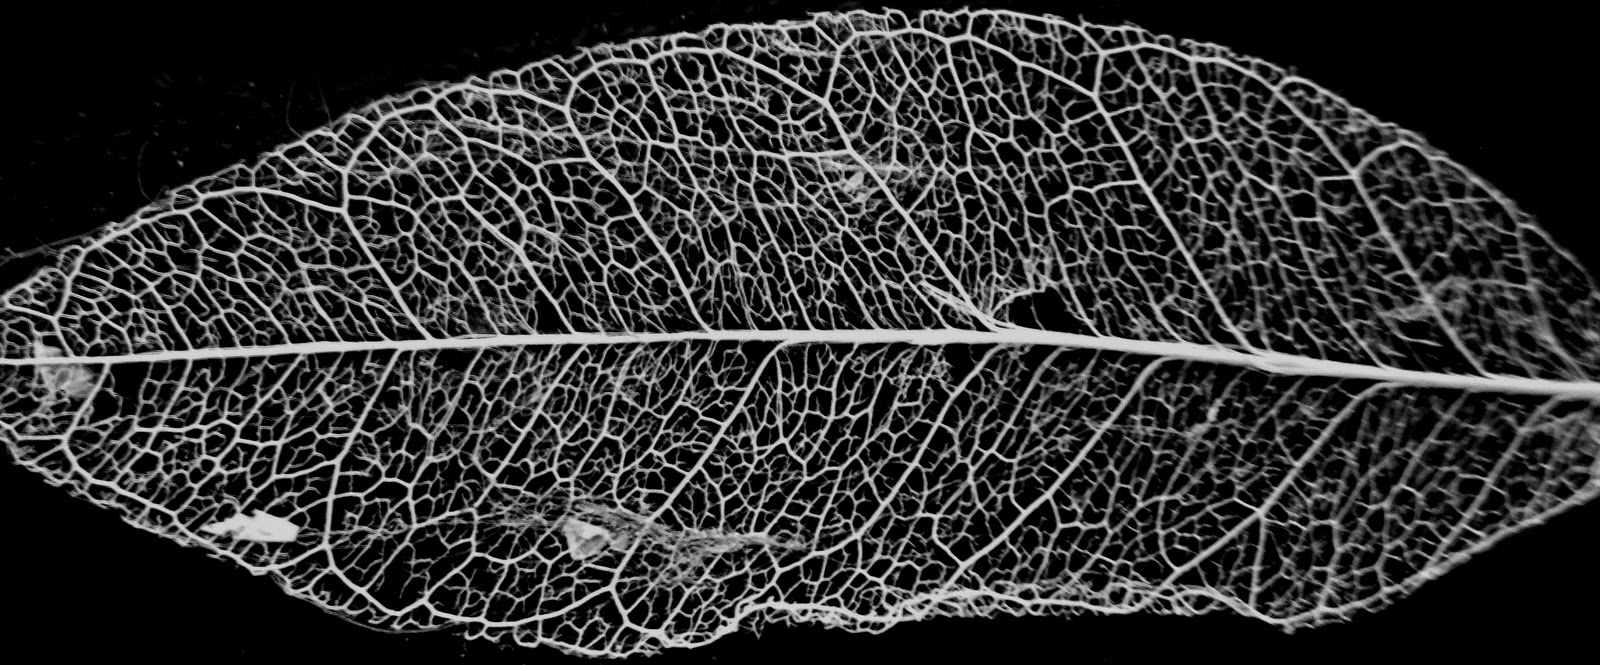
\includegraphics[width=5cm]{pictures/list.jpg}
\caption{Voronoiovy diagramy v přírodě - na kůži žirafy, na křídle vážky a na žilkování listu}
\end{figure}


Tato dokumentace je však zaměřena na triangulaci. Existuje mnoho druhů triangulace v závislosti na geometrické konstrukci - Greedy triangulace, Minimum Weight Triangulation, Constrained triangulation, nejčastěji používaná je však Delaunay triangulace.  Zjednodušeně si lze Delaunyho triangulaci představit tak, že zvolíme tři body, kterým opíšeme kružnici. Pokud uvnitř kružnice neleží žádný další bod, vytvoři se trojúhelník. Pokud se uvnitř bod nachází, zvolí se jiné tři body. Tato triangulace je jednoznačná, pokud žádné čtyři body neleží na kružnici. Trojúhelníky vzniklé Delaunyho triangulací se nejvíce blíží rovnostranným trojúhelníkům. \\
\\
V dnešní době se kromě analýzy prostorových dat využívá Delaunyho triangulace a Voronoiovy diagramy například v grafice. Takto vytvořené obrazy jsou nazývaný Delaunayho rastry (The Delaunay Raster). Autoři takovýchto děl jsou schopni pomocí Delaunay triangulace sami vytvářet obrazy, případně převést existující obraz na triangulaci. [Zdroj: 4]

\begin{figure}[h!]
\centering
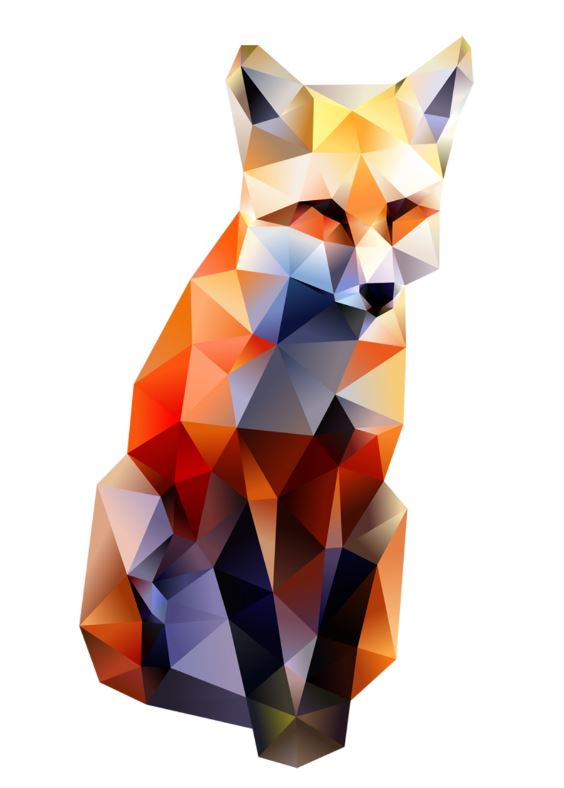
\includegraphics[width=7cm]{pictures/liska.jpg}
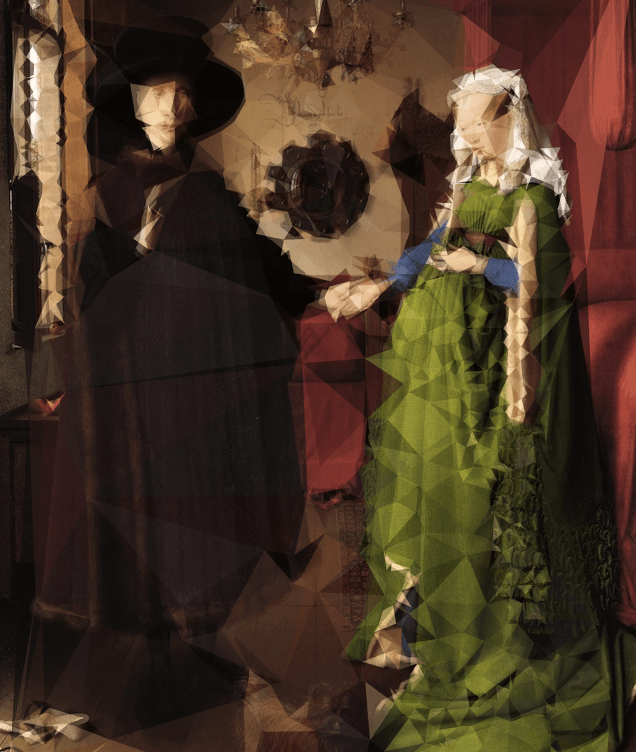
\includegraphics[width=7cm]{pictures/jan_van_eyck.png}
\caption{Použití Delaunayho triangulace v grafice - na vytvořeném novém obrázku lišky a na přepracování obrazu od Jana van Eycka}
\end{figure}

\section{Popis použitých algoritmů}
Existuje několik způsobů jak vytvořit triangulaci s různými kritérii. Obecně lze metody triangulace rozdělit na dvě skupiny. Jednou je skupina triangulací dle geometrické konstrukce. Mezi tyto triangulace se řadí Greedy triangulace, Delaunay triangulace, Minimum Weight triangulace, Constrained triangulace (triangulace s povinnými hranami) a datově závislé triangulace. Případně lze triangulace rozdělit dle použitých kritérií, tedy na lokálně optimální triangulace, globálně optimální triangulace a multikriteriálně optimalizované triangulace. \\
\\
V této úloze jsme se zabývali Delaunay triangulací pomocí metody inkrementální konstrukce. Další metody přímé konstrukce Delaunay triangulace jsou např. metoda lokálního prohazování, inkrementálního vkládání, Divide and Conquer (rozděl a panuj) či Sweep Line (zametací přímka). Pro nepřímou konstrukci se využívají Voronoiho diagramy, v praxi však tento způsob není používaný. 

\subsection{Delaunay triangulace}
Delaunay triangulace je nejčastěji používanou triangulací při tvorbě digitálního modelu terénu. Delaunay triagulaci lze provádět v rovině i v prostoru.\\
\\
Triangulace byla realizována pomocí metody inkrementální konstrukce. Tento algoritmus je založen na postupném hledání bodu, který k bodům hrany tvoří minimální opsanou kružnici. Každá hrana je orientovaná a bod se hledá pouze v její levé polorovině.\\
\\
Je-li nalezen bod s výše uvedeným kritériem, vytvoří se dvě nové hrany, které jsou přidány do triangulace. Nenalezne-li se daný bod, prohodí se orientace hrany a hledání pokračuje.\\
\\
Hrany, které nebyly zlegalizovány (nebyl k nim ještě nalezen třetí bod), jsou ukládány do struktury Active Edge List (AEL). Pokud k dané hraně byl nalezen třetí bod, hrana se ze struktury odstraní. Než je hrana vložena do struktury, kontroluje se, zda hrana už ve struktuře není s opačnou orientací. Pokud je, hrana se nevloží. Algoritmus probíhá do té doby, dokud není struktura AEL prázdná.

\subsubsection{Vlastnosti Delaunay triangulace}

\begin{enumerate}
\item Uvnitř opsané kružnice libovolného trojúhelníku triangulace neleží žádný jiný bod.
\item Maximalizuje minimální úhel, avšak neminimalizuje maximální úhel v trojúhelníku.
\item Vůči kritériu minimálního úhlu je lokálně i globálně optimální.
\item Triangulace je jednoznačná, pokud čtyři body neleží na kružnici.
\end{enumerate}

\subsubsection{Implementace metody}
\begin{enumerate}
\item Nalezení pivota q s minimální souřadnicí X:  $ q = min(x_i) $ 
\item Hledání nejbližšího bodu bodu: $ ||p_1 - q||_2 = min  $
\item Vytvoření první hrany: $ e = (q, p_1) $ 
\item Hledání Delaunay bodu: $ \underline{p} = argmin_{\forall p_i \in \sigma_L (e)} r'(k_i); k_i = (a, b, p_i); e = (a, b)$ 
\subitem Při nenalezení Delaunay bodu změna orientace: $ \nexists \underline{p} : e \leftarrow (p_1, q);$ go to 4. 
\item Vytvoření zbývajících hran trojúhelníka: $ e_2 = (p_1,  \underline{p}); e_3 = ( \underline{p} , q) $
\item Přidání hran trojúhelníka do DT:  $ DT \leftarrow e; DT \leftarrow e_2; DT \leftarrow e_3  $  
\item Přidání hran trojúhelníka do AEL:  $ AEL \leftarrow e; AEL \leftarrow e_2; AEL \leftarrow e_3  $  
\item Dokud není AEL prázdný proveď:
\subitem Hledání Delaunay bodu k hraně z AEL (viz 4).
\subitem Pokud Delaunay bod existuje. $ if \exists  \underline{p}$
\subsubitem Vytvoření zbývajících hran trojúhelníku:   $ e_2 = (p_1,  \underline{p}); e_3 = ( \underline{p} , q) $
\subsubitem Pokud nová hrana není v AEL, přidej.
\end{enumerate}

\subsection{Vrstevnice}
Vrstevnice jsou půdorysným obrazem průsečných čar vodorovných rovin s terénem, přičemž jejich nadmořská výška je bezezbytku dělitelná zvoleným základem. Existují 4 druhy vrstevnic - základní, zvýrazněné, doplňkové a pomocné. Základní vrstevnice jsou vyobrazené tenkou křivkou a jejich rozestup je roven intervalu vrstevnic. Zvýrazněné vrstevnice jsou značeny tučně a obvykle jsou voleny jako pětinásobek základního intervalu. Doplňkové vrstevnice mají většinou poloviční či čtvrtinový interval a znázorňují se čárkovaně nejčastěji v místech  plochého terénu. Pomocné vrstevnice slouží jen pro orientaci v místech, kde může docházet k podstatným změnám terénu (sesuvná území, lomy). \\
\\
Při popisu vrstevnic existuje několik kartografických zásad. Pozice textu by měla symbolizovat terén, tedy hlava popisu směrem do kopce a pata do klesání. Dále by měl být popis zobrazen stejným způsobem jako popisovaná vrstevnice (barva, tučně apod). Z důvodu čitelnosti je nutné vrstevnici v místě popisu přerušit. Je vhodné, aby byl popis rovnoměrně rozmístěn po mapovém poli. \\
\\
Existují dva základní způsoby konstrukce vrstevnic. U lineární interpolace je rozestup vrstevnic mezi dvěma body konstantní, tedy i spád. Při konstrukci vrstevnic hledáme průsečnici vodorovné roviny o výšce Z a rovinu trojúhelníka triangulace. V úloze byly vrstevnice konstruovány lineární interpolací.\\

\subsubsection{Implementace metody}
\begin{enumerate}
\item Pro všechny hrany trojúhelníku t: $ \forall e_i \in t: $
\item Hrana náleží rovině vrstevnice z: $ (z - z_i) \cdot (z - z_{i+1}) = 0 \rightarrow e_i \in \rho $
\item Hrana nenáleží rovině vrstevnice z: $ (z - z_i) \cdot (z - z_{i+1}) < 0 \rightarrow e_i \not \in \rho $
\item Hrana je průnikem roviny vrstevnice z: $ (z - z_i) \cdot (z - z_{i+1}) < 0 \rightarrow e_i \cap \rho $
\subitem Výpočet polohových souřadnic: 
$$  x = \frac{(x_2 - x_1)}{(z_2 - z_1)} (z - z_1) + x_1 $$ 
$$  y = \frac{(y_2 - y_1)}{(z_2 - z_1)} (z - z_1) + y_1 $$ 
\subitem Vytvoř hranu tvořící vrstevnici.

\end{enumerate}

\subsection{Sklon terénu}
Skon terénu je definován jako úhel mezi normálovým vektorem (0,0,1) a normálovým vektorem roviny trojúhelníku. Pro výpočet je dostačující vypočítat směrové vektory v trojúhelníku. Do výpočtu vstupuje normálový vektor (0, 0, 1), jehož norma je rovna jedné a který v čitateli argumentu funkce arcus cosinus ponechá pouze Z část normálového vektoru.


\subsubsection{Implementace metody}
\begin{enumerate}
\item Pro všechny trojúhelníky triangulace: $ \forall t_i \in DT: $
\subitem Výpočet normálového vektoru roviny trojúhelníku: \\
 $$ n_t = (u_y \cdot v_z - u_z \cdot v_y)^2 - (u_x \cdot v_z - u_z \cdot v_x)^2  + (u_x \cdot v_y - u_y \cdot v_x)^2 $$
\subitem Kde:
$$  u_x = \Delta x_2, x_1; u_y = \Delta y_2, y_1; u_z = \Delta z_2, z_1;$$
$$  v_x = \Delta x_2, x_3; u_y = \Delta y_2, y_3; u_z = \Delta z_2, z_3;$$
\item Výpočet sklonu: $ \varphi = arccos \frac{n_z}{|n_t|} $

\end{enumerate}

\subsection{Expozice terénu}
Expozice terénu je definována jako azimut k průmětu normálového vektoru roviny trojúhelníku do roviny x, y. Expozice má významný vliv na energetické poměry, neboť znázorňuje jednotlivé dopady slunečního záření, s čímž souvisí i výpar vody v oblasti. 

\subsubsection{Implementace metody}
\begin{enumerate}
\item Pro všechny trojúhelníky triangulace: $ \forall t_i \in DT: $
\subitem Výpočet x a y části normálového vektoru: \\
$$ n_x = (u_y \cdot v_z - u_z \cdot v_y) $$
$$ n_y = -(u_x \cdot v_z - u_z \cdot v_x) $$
\subitem Kde:
$$  u_x = \Delta x_2, x_1; u_y = \Delta y_2, y_1; u_z = \Delta z_2, z_1;$$
$$  v_x = \Delta x_2, x_3; u_y = \Delta y_2, y_3; u_z = \Delta z_2, z_3;$$
\item Výpočet expozice: $ A =atan2( \frac{n_x}{n_y}) $
\end{enumerate}

\

Pro výpočet expozice byla použita funkce atan2, která automaticky určí i daný kvadrant, a tím je vypočtený úhel korektní směrnicí.

\section{Informace o bonusových úlohách}
\subsection{Výběr barevných stupnic při vizualizaci sklonu a expozice}
V rámci této bonusové úlohy byly definovány barevné stupnice pro zobrazení sklonu a expozice. Pro sklon byly zvoleny odstíny šedi. Pro zobrazení šedé barvy v režimu RGB je typické to, že všechny tři složky mají stejné číslo. Bylo tedy snadné rozdělit interval 256 (jedná se o osmi bitovou hloubku) dle intervalu, ve kterém vychází sklon terénu.\\
\\
Pro vyznačení expozice byly voleny syté barvy. Inspirací byla barevná škála v programu ArcGIS, přesto byly barvy zvoleny tak, aby byly asociativní se směrem, který reprezentují.

\subsection{Algoritmus pro automatické generování terénních tvarů}
V aplikaci je možnost automatického generování terénních tvarů. Na výběr je kupa, údolí, hřbet, grid, sedlo a spočinek. Přesto, že grid neoznačuje žádný terénní tvar, byl mezi možnosti přidán z toho důvodu, abychom demonstrovali špatnou implementaci takovéhoto rozmístění bodů. Definice a anglická pojmenování jednotlivých útvarů byla použita ze stránky VÚGTK. [Zdroj: 5]

\subsubsection{Kupa}
Jedná se o takový terénní útvar, který je vyvýšený nad okolní terén. Běžně bývá tento tvar označován jako kopec či hora. V rámci aplikace je zvoleno pojmenování Hill. \\
\\
Kupa byla generována klasickým způsobem jako elipsa, pro Z souřadnici bylo však navolena, že hodnota postupně klesá. Pro vhodné zobrazení byl krok klesání zvolen 20.\\
\\
$ X = X_0 + a * cos(\phi)$ \\
$ Y = Y_0 + b * sin(\phi) $ \\
$ Z = Z_0 - j* 20 $ \\


\subsubsection{Údolí}
Jedná se o takový terénní útvar, který se vyznačuje protáhlým tvarem, jehož okraje jsou lemovány vyvýšeným terénem. V rámci aplikace je použito označení Valley. \\
\\
Pro údolí byly vygenerovány přímky od nichž se v zadaném kroku vytváří nové přímky s konstantně stoupající hodnotou výšky. V uvedených vzorcích jsou p1 a p2 označení pro vzniklé přímky.\\
\\
$ X_{p1} = X_0 + a $ \\
$ Y_{p1} = Y_0 + i * 10 $ \\
$ Z_{p1} = Z_0 + a $ \\
\\
$ X_{p2} = X_0 - a $ \\
$ Y_{p2} = Y_0 + i * 10 $ \\
$ Z_{p2} = Z_0 + a $ \\

\subsubsection{Hřbet}
Hřbet je protáhlá vypuklá terénní plocha se zaoblenou vrcholovou částí. V aplikace je pojmenován jako Ridge. \\
\\
Hřbet byl generován podobným způsobem jako údolí, s tím rozdílem, že výška postupně nestoupá, ale klesá. \\
$ X_{p1} = X_0 + a $ \\
$ Y_{p1} = Y_0 + i * 10 $ \\
$ Z_{p1} = Z_0 - a $ \\
\\
$ X_{p2} = X_0 - a $ \\
$ Y_{p2} = Y_0 + i * 10 $ \\
$ Z_{p2} = Z_0 - a $ \\

\subsubsection{Sedlo}
Sedlo je místo v krajině, které se nachází mezi dvěma vrcholy, z něhož na dvě strany svahu sestupují do údolí a na ostatní dvě stoupají směrem k vrcholkům. U vysokých hor se sedlo často označuje jako průsmyk. V aplikace je použito označení Saddle. \\
\\
Generování sedla zahrnovalo vygenerování dvou vrcholů a dvou ďolíků. Podstatné bylo rozmístění. To se regulovalo zadanými pevnými souřadnicemi vrcholů, případně děr. následně byly kolem těchto středu generovány elipsy s klesající/rostoucí výškou. \\
\\
Tvorba vrcholků: \\
$ X = X_0 + i * rand\%(70) * cos(j*\phi) + rand\%(20) $ \\
$ Y =  Y_0 + i * rand\%(70) * sin(j*\phi) + rand\%(20) $ \\
$ Z = Z_0 - i * 50 $ \\
\\
Tvorba děr: \\
$ X = X_0 + i * rand\%(70) * cos(j*\phi) + rand\%(20) $ \\
$ Y =  Y_0 + i * rand\%(70) * sin(j*\phi) + rand\%(20) $ \\
$ Z = Z_0 + i * 50 $ \\

\subsubsection{Spočinek}
Spočinek je vodorovná nebo mírně skloněná část terénního reliéfu na svahovém hřbetu nebo svahu. V aplikaci lze spočinek vygenerovat názvem Col Topographic. \\
\\
Tvorba spočinku se náhodně vytváří proto, že v kódu je tvorba nových bodů pouze v jednom kvadrantu a vzhledem k pravděpodobnosti blízkosti některých bodů se při generování vytváří v některých situacích spočinek. Tato tvorba je však zcela náhodná a neřízená, autoři si za to nenárokují žádné body z této úlohy, spočinek byl v úloze ponechán z toho důvodu, že na něm lze demonstrovat nefunkčnost tvorby vrstevnic, ale funkčnost vytvořeného sklonu a expozice. \\
\\
Tvorba spočinku: \\
$ X = X_0 + i * rand\%(100) * cos(j*\phi) + rand\%(50) $ \\
$ Y =  Y_0 + i * rand\%(150) * sin(j*\phi) + rand\%(50) $ \\
$ Z = Z_0 - i * 50 $ \\


\section{Vstupní data}
V aplikaci lze generovat jednotlivé útvary terénu a nebo lze importovat data ve formátu .txt. Automatická tvorba bodů kurzorem byla odstraněna.\\

Vzor vstupních dat ve formátu .txt\\
 748720.120    1048636.300     306.100\\
 748720.750    1048636.130     305.940\\
 748721.600    1048635.700     306.080\\
 748721.610    1048628.180     305.570\\

\section{Výstupní data}
Výstupem je grafická aplikace, která na vstupních datech vytvoří Delaunay triangulaci, se zvoleným krokem vykreslí vrstevnice a následně je možné zobrazit sklon či expozici terénu. 

\clearpage
\section{Aplikace}

\begin{figure}[h!]
\centering
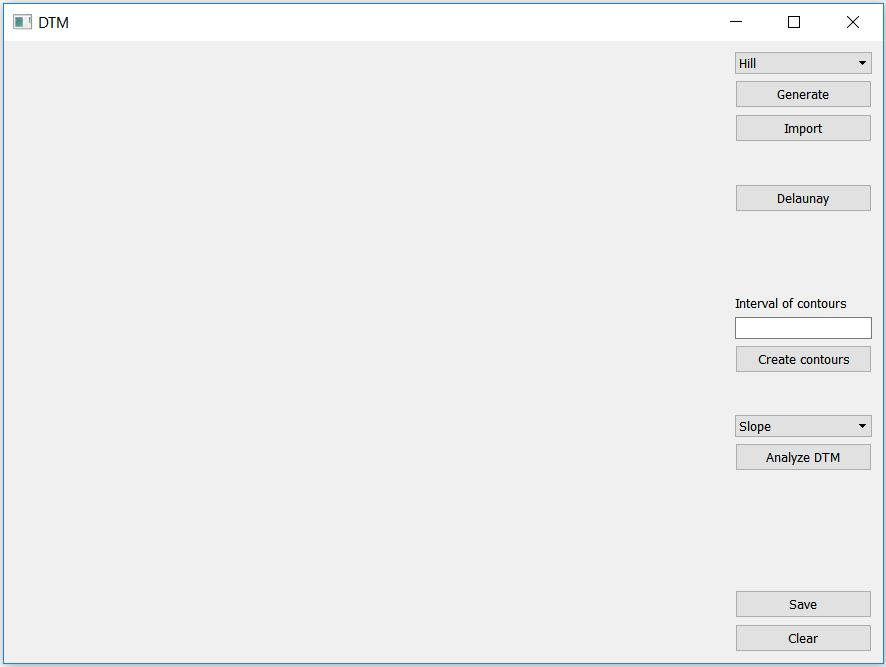
\includegraphics[width=10cm]{pictures/vstup.jpg}
\caption{Vstupní vzhled aplikace}
\end{figure}

\begin{figure}[h!]
\centering
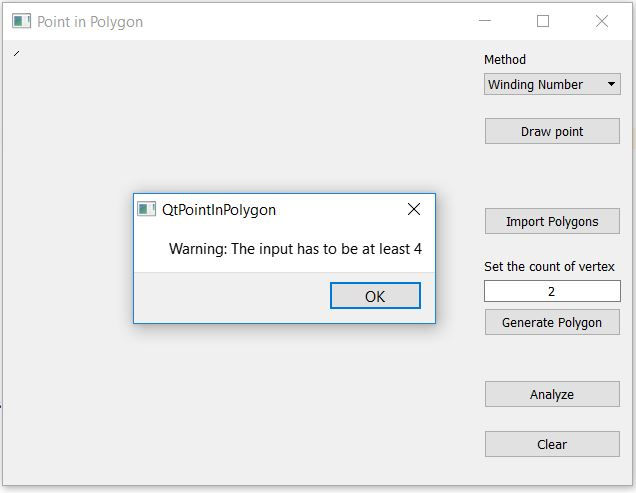
\includegraphics[width=10cm]{pictures/warning.jpg}
\caption{Varování při nesprávném vstupu intervalu souřadnic (zde 1.0, je nutné zadávat ve formátu celého čísla)}
\end{figure}

\begin{figure}[h!]
\centering
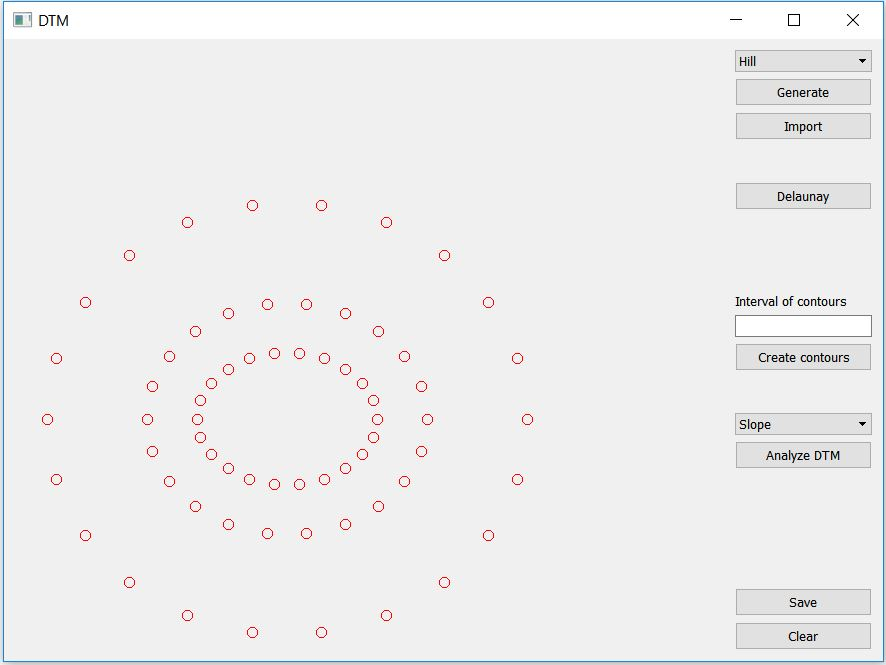
\includegraphics[width=10cm]{pictures/hill.jpg}
\caption{Vygenerované body znázorňující kupu}
\end{figure}

\begin{figure}[h!]
\centering
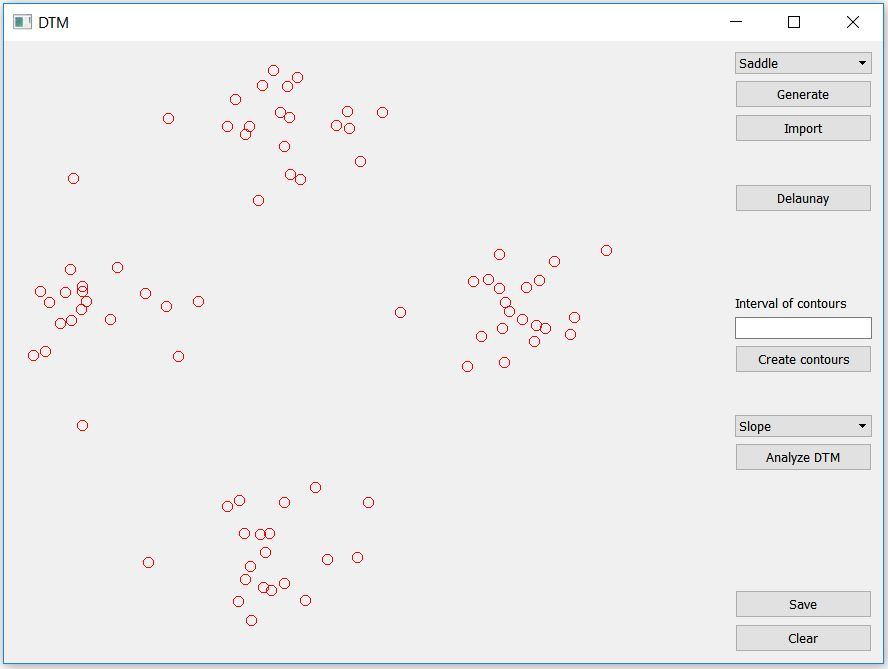
\includegraphics[width=10cm]{pictures/saddle.jpg}
\caption{Vygenerované body znázorňující sedlo}
\end{figure}

\begin{figure}[h!]
\centering
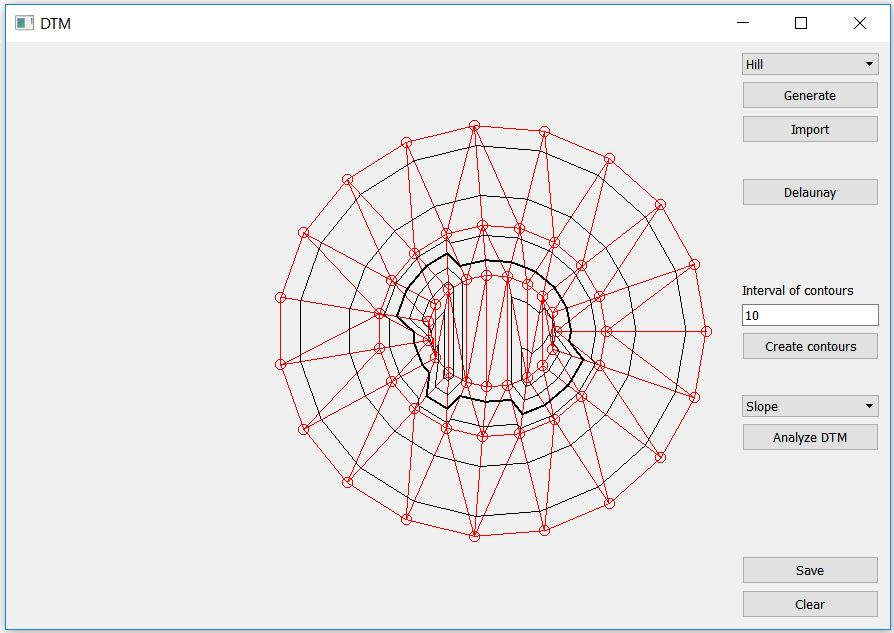
\includegraphics[width=10cm]{pictures/hill_bad.jpg}
\caption{Špatně vykreslené vrstevnice kupy}
\end{figure}

\begin{figure}[h!]
\centering
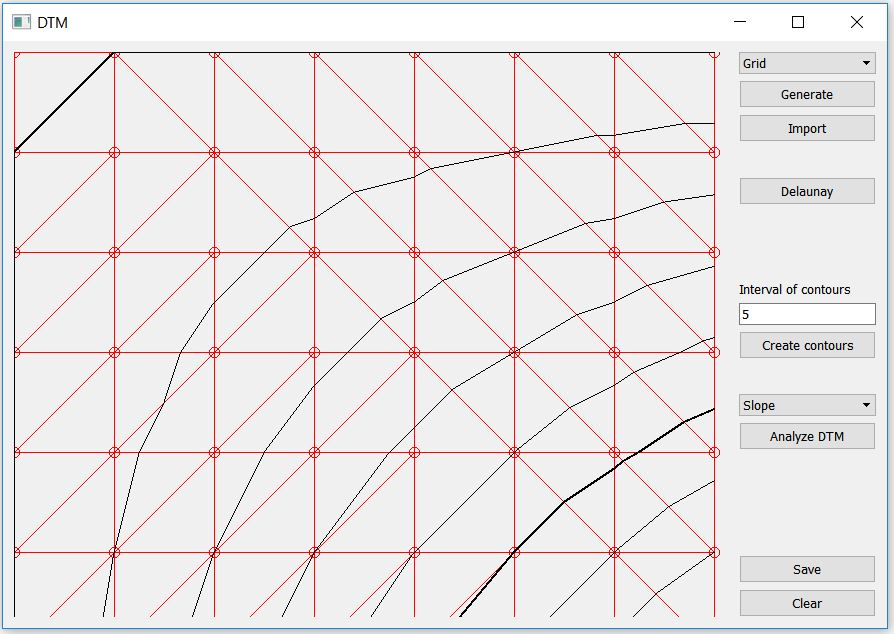
\includegraphics[width=10cm]{pictures/grid_ok.jpg}
\caption{Vrstevnice pro grid jsou vykresleny korektně}
\end{figure}

\begin{figure}[h!]
\centering
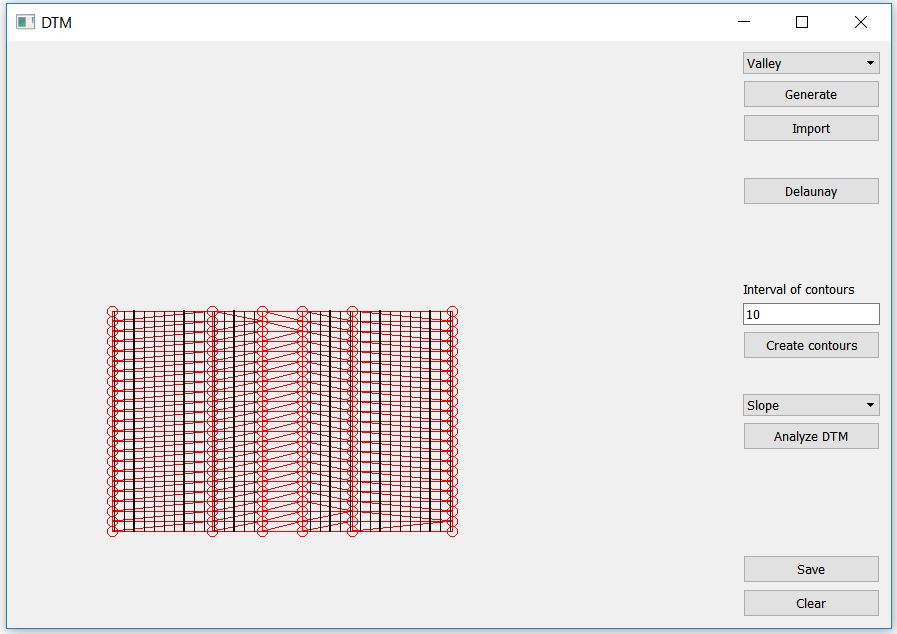
\includegraphics[width=10cm]{pictures/valley_ok.jpg}
\caption{Vrstevnice pro údolí vykresleny korektně}
\end{figure}

\begin{figure}[h!]
\centering
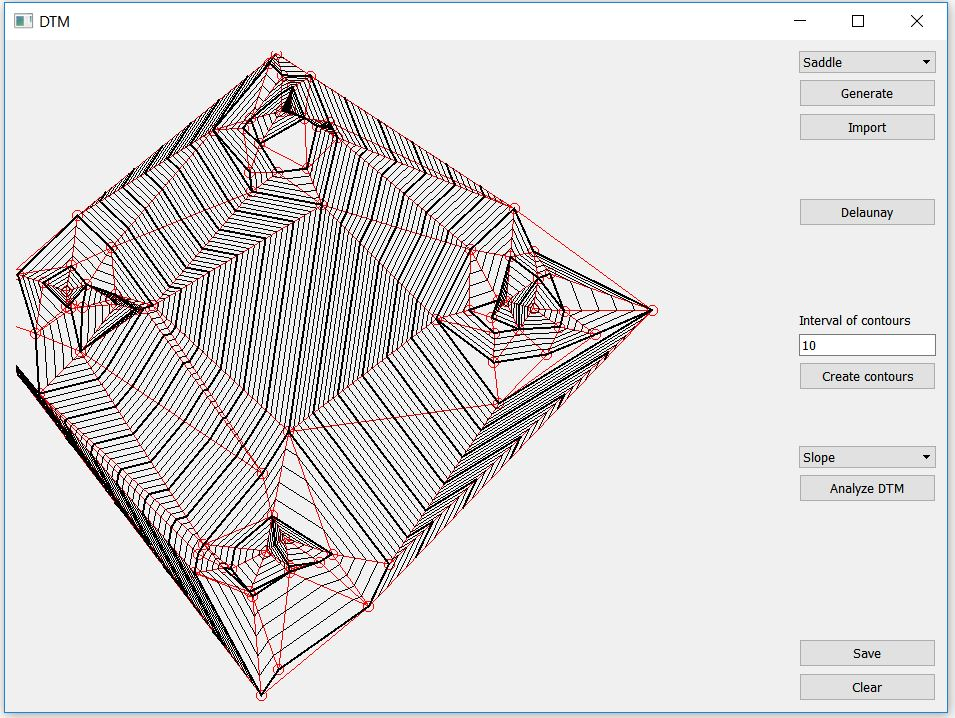
\includegraphics[width=10cm]{pictures/saddle_bad.jpg}
\caption{Nekorektně vykreslené vrstevnice pro sedlo}
\end{figure}

\begin{figure}[h!]
\centering
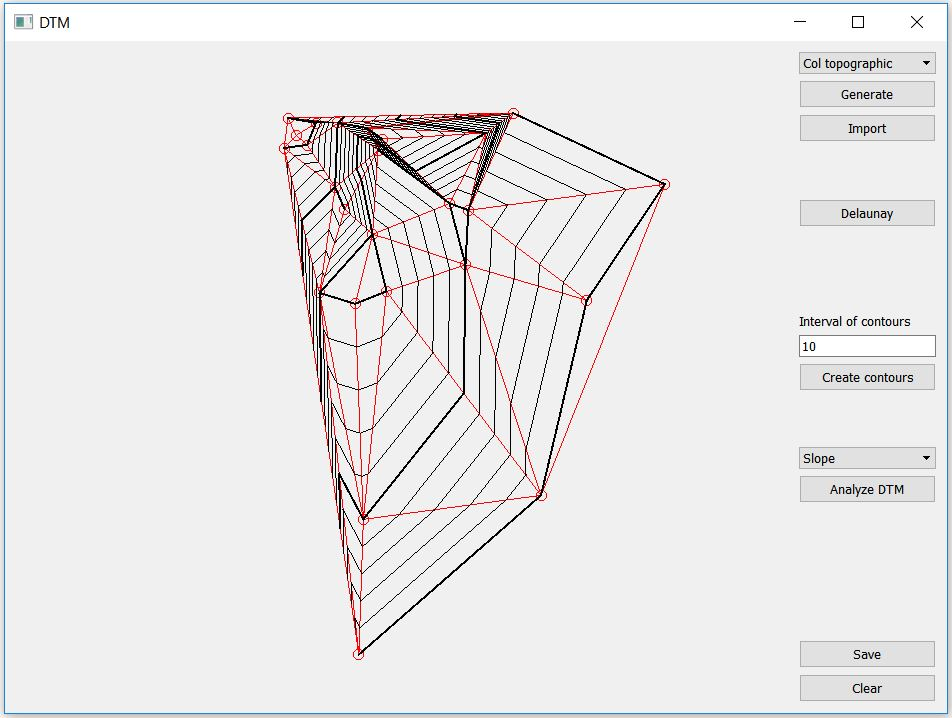
\includegraphics[width=10cm]{pictures/spocinek_nicmoc.jpg}
\caption{Nekorektně vykreslené vrstevnice pro spočinek}
\end{figure}

\begin{figure}[h!]
\centering
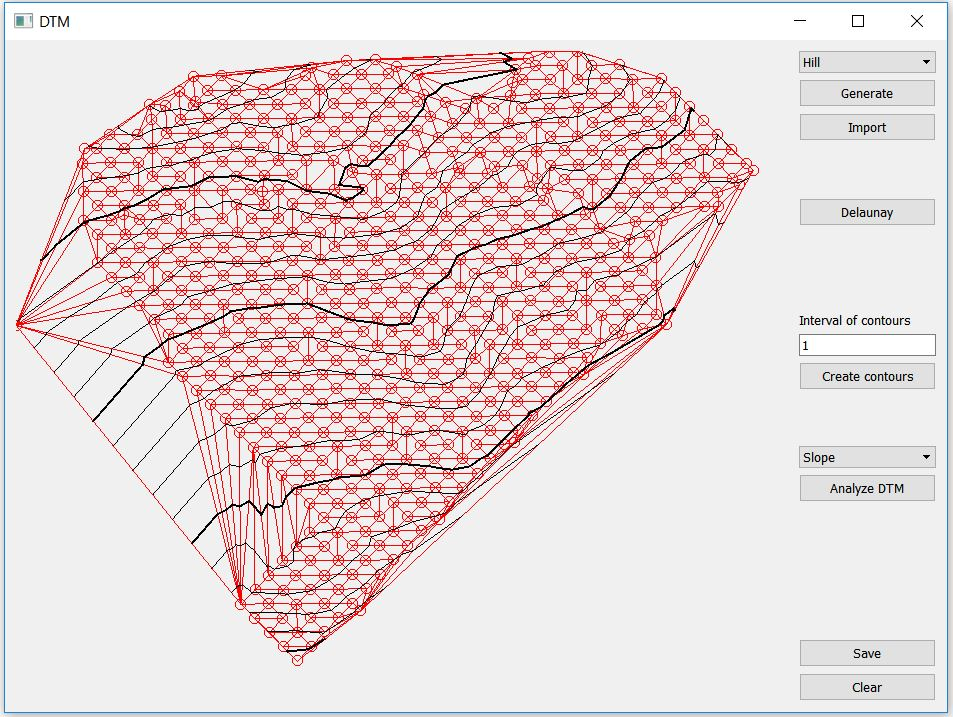
\includegraphics[width=10cm]{pictures/imported.jpg}
\caption{Vygenerované vrstevnice pro importovaná data}
\end{figure}

\begin{figure}[h!]
\centering
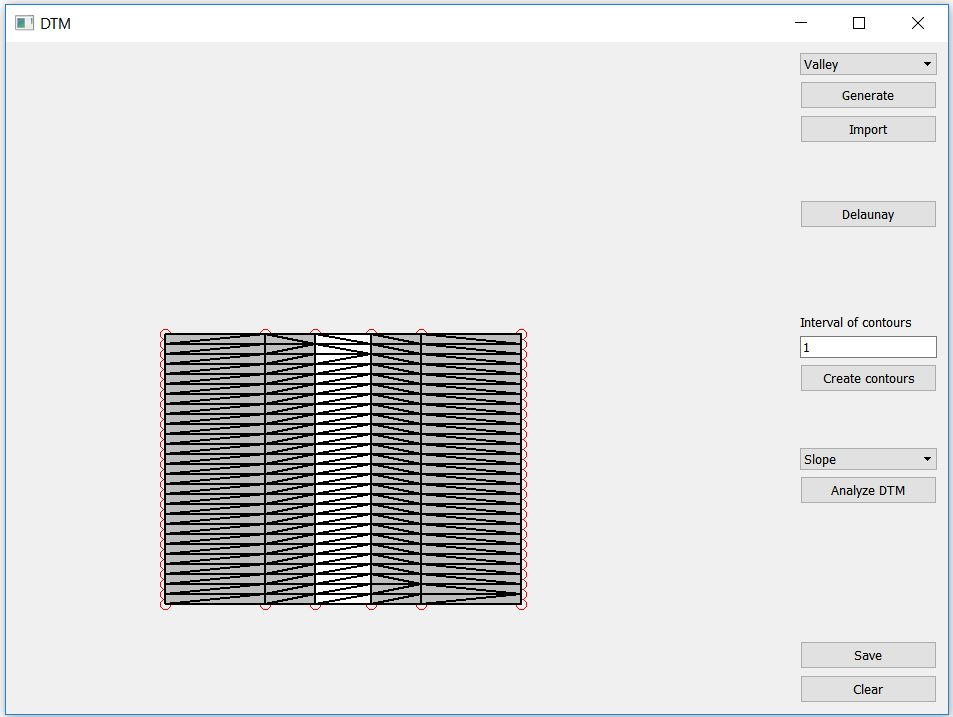
\includegraphics[width=10cm]{pictures/valley_sklon.jpg}
\caption{Zobrazení sklonu pro údolí korektní}
\end{figure}

\begin{figure}[h!]
\centering
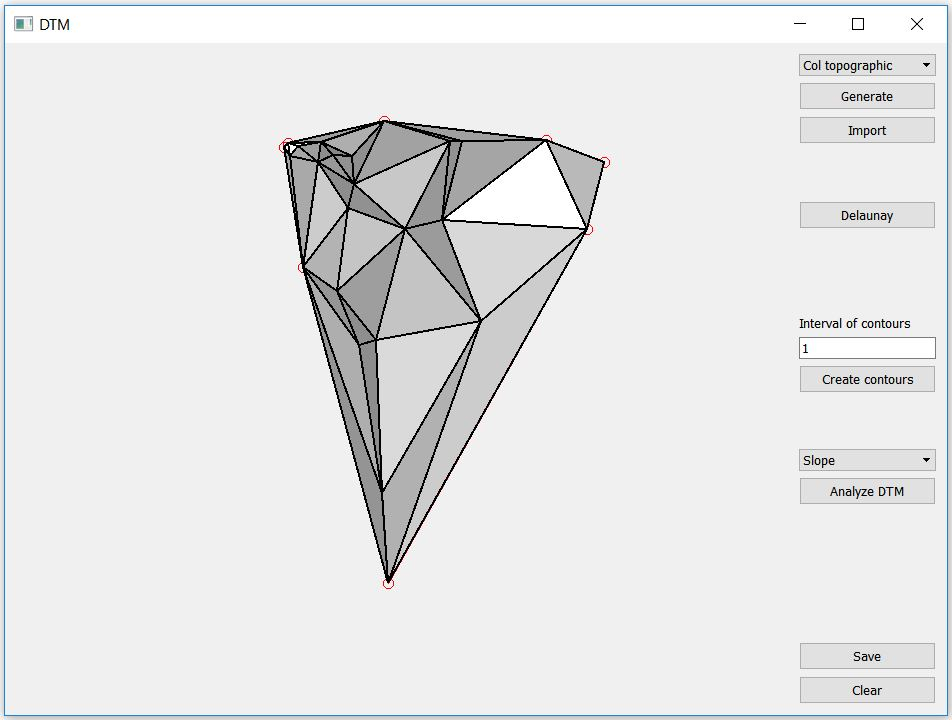
\includegraphics[width=10cm]{pictures/spocinek_sklon.jpg}
\caption{Oblast spočinku vykreslena správně}
\end{figure}

\begin{figure}[h!]
\centering
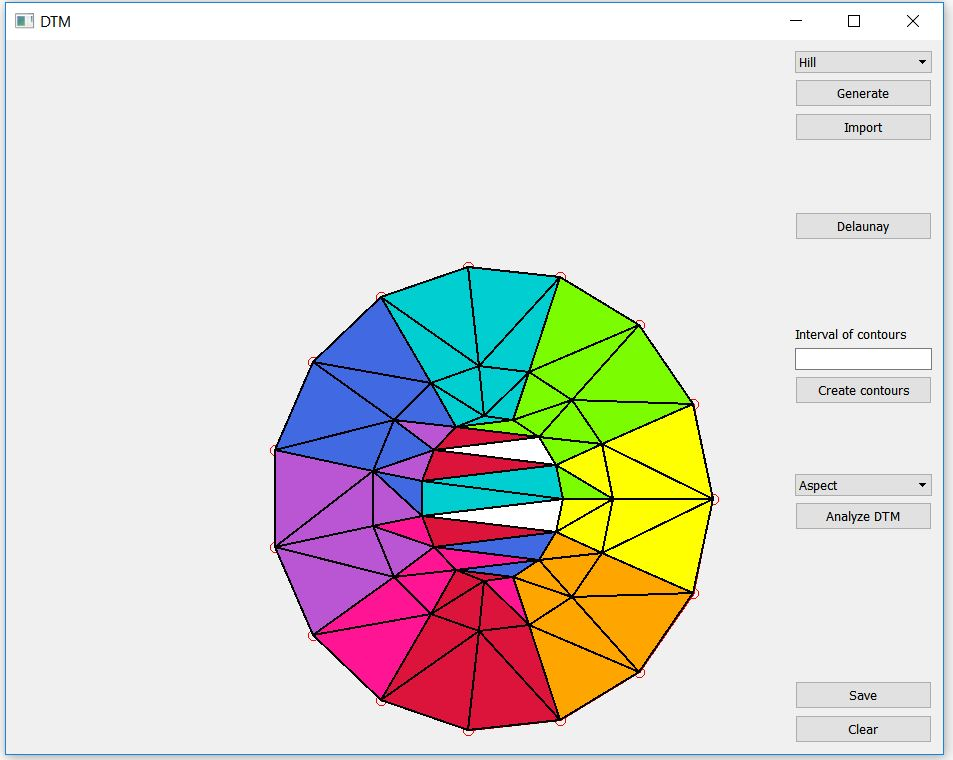
\includegraphics[width=10cm]{pictures/hill_aspect.jpg}
\caption{Expozice pro kupu vykreslena téměř správně až na oblasti, kde selhávaly i vrstevnice}
\end{figure}

\begin{figure}[h!]
\centering
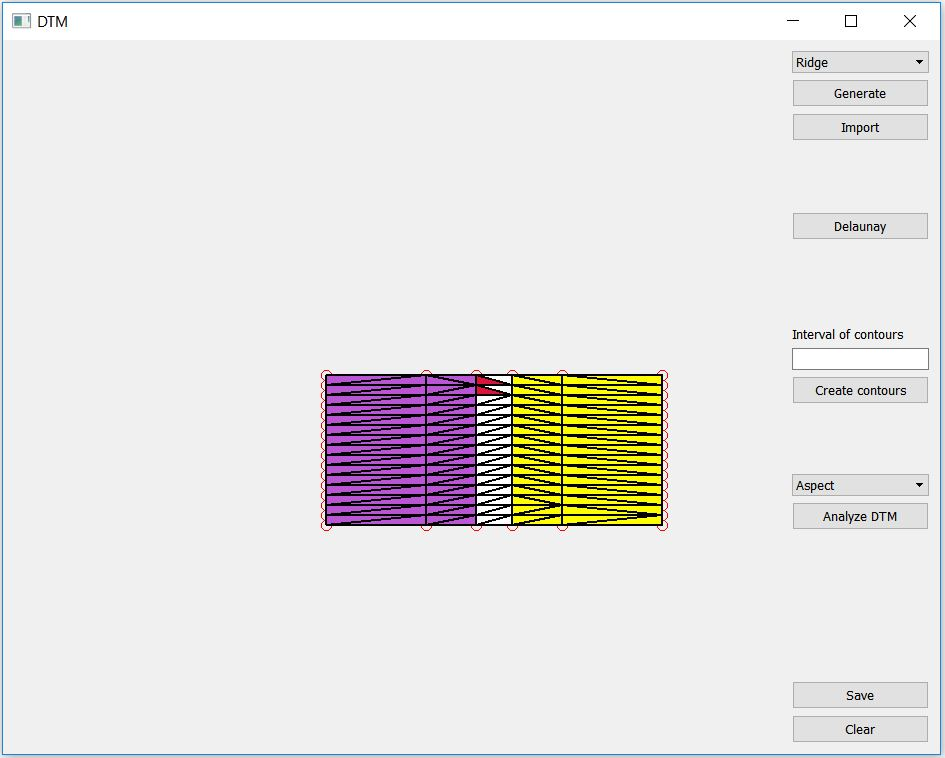
\includegraphics[width=10cm]{pictures/ridge_expozice.jpg}
\caption{Expozice pro hřbet nezobrazeny korektně}
\end{figure}

\begin{figure}[h!]
\centering
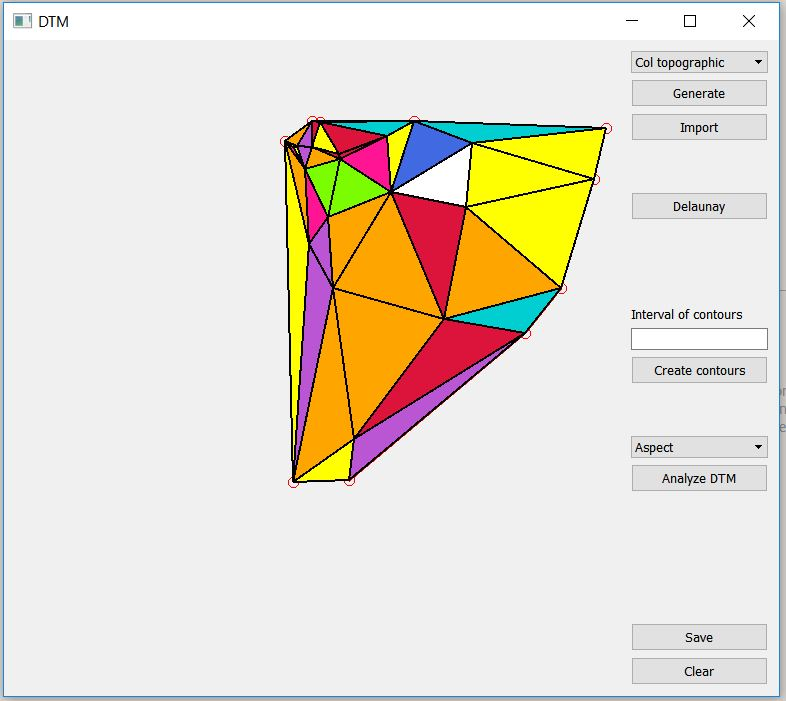
\includegraphics[width=10cm]{pictures/spocinek_expozice.jpg}
\caption{Korektně vytvořená expozice pro spočinek}
\end{figure}

\begin{figure}[h!]
\centering
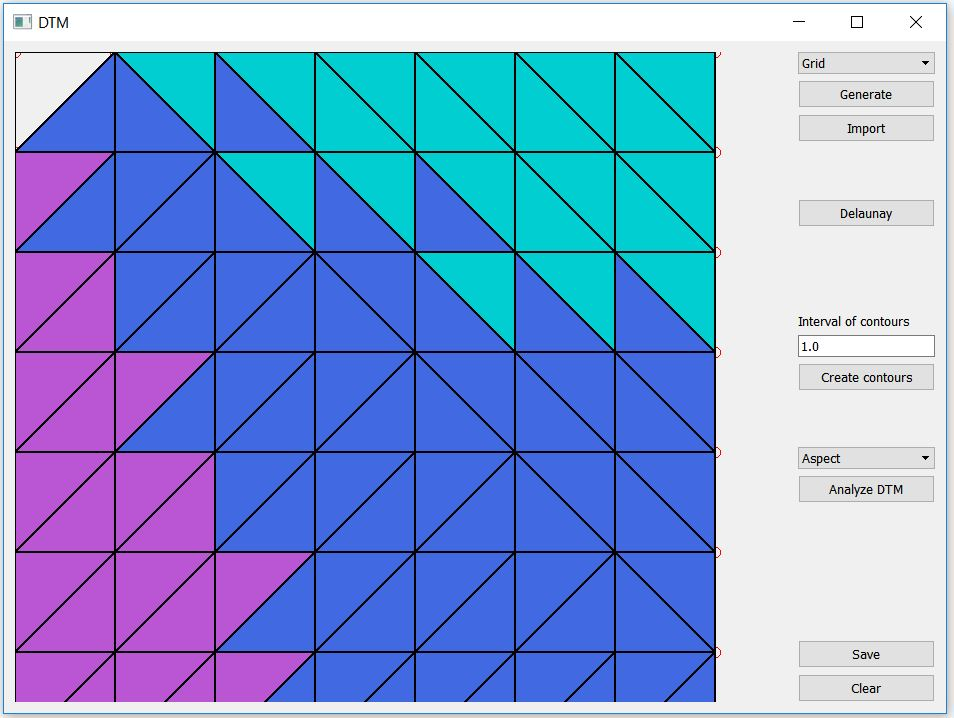
\includegraphics[width=10cm]{pictures/grid_aspect.jpg}
\caption{Expozice pro grid nezobrazeny korektně}
\end{figure}

\begin{figure}[h!]
\centering
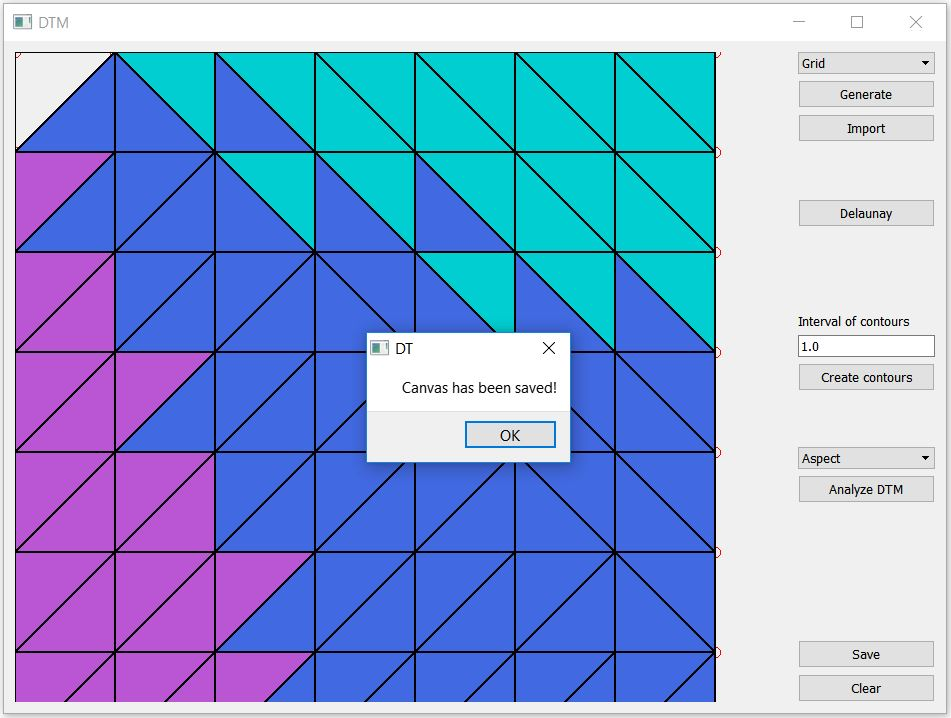
\includegraphics[width=10cm]{pictures/saved.jpg}
\caption{Ukládání zájmové oblasti}
\end{figure}

\begin{figure}[h!]
\centering
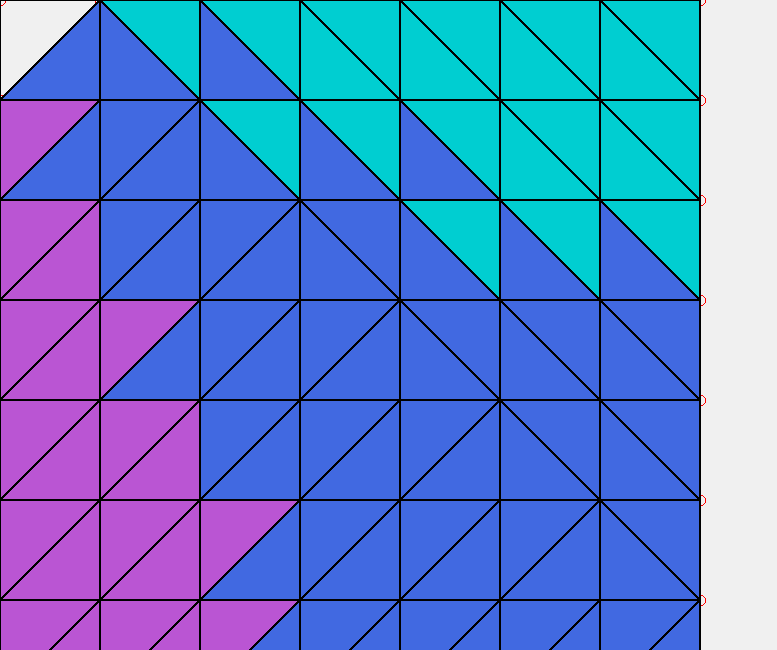
\includegraphics[width=10cm]{pictures/exported.png}
\caption{Pro ukázku vyexportovaná zájmová oblast}
\end{figure}

\clearpage



\section{Dokumentace}
\subsection{Třídy}
\subsubsection{Algorithms}
Třída Algorithms obsahuje několik metod. Metody jsou určeny pro výpočty použitých algoritmů.
\\

\textbf{double distance(QPoint3D p1, QPoint3D p2)}\\
Metoda, jejíž návratová hodnota je typu double, vrací velikost spojnice mezi dvěma body.
\\

\textbf{TPosition getPointLinePosition(QPoint \&q, QPoint \&a, QPoint \&b)}\\
Tato metoda slouží k určení pozice bodu q vůči linii tvořené body a, b. Výstupem metody je LEFT, RIGHT nebo ON.\\

\textbf{double getCircleRadius(QPoint3D \&p1, QPoint3D \&p2, QPoint3D \&p3, QPoint3D \&c)}\\
Metoda jejíž návratová hodnota je typu double, vrací velikost poloměru kružnice tvořené třemi vstupními body.\\

\textbf{int getNearestPoint(QPoint3D \&p, std::vector\textless QPoint3D\textgreater \&points)}\\
Tato metoda slouží k nalezení indexu nejbližšího bodu k bodu p.\\

\textbf{int getDelaunayPoint(QPoint3D \&s, QPoint3D \&e, std::vector\textless QPoint3D \textgreater \&points)}\\
Tato metoda slouží k nalezení indexu bodu, který splňuje Delaunay vlastnosti.\\

\textbf{std::vector\textless Edge \textgreater DT(std::vector \textless QPoint3D \textgreater \&points)}\\
Metoda vytváří nad vektorem bodů Delaunay triangulaci, která je reprezentována jako vektor hran.\\

\textbf{QPoint3D getContourPoint(QPoint3D \&p1, QPoint3D \&p2, double z)}\\
Metoda vypočte průsečík hrany, tvořenou 3D body p1 a p2, a rovinou definovanou Z souřadnicí.\\

\textbf{std::vector\textless Edge \textgreater createContours(std::vector\textless Edge \textgreater \&dt, $double z_min, double z_max, double dz$)}\\
Metoda z triangulace dt v zadaném intervalu v ose Z $<z_{min} ; z_{max}>$ s intervalem vrstevnic dz vrátí vektor hran definující vrstevnice.\\

\textbf{double getSlope(QPoint3D \&p1, QPoint3D \&p2, QPoint3D \&p3)}\\
Tato metoda slouží k vypočetní hodnoty sklonu trojúhelníku definovanému 3D body p1, p2 a p3.\\

\textbf{double getAspect(QPoint3D \&p1, QPoint3D \&p2, QPoint3D \&p3)}\\
Tato metoda slouží k vypočetní hodnoty expozice trojúhelníku definovanému 3D body p1, p2 a p3.\\

\textbf{std::vector\textless Triangle\textgreater analyzeDTM(std::vector\textless Edge \textgreater \&dt)}\\
\\

\textbf{std::vector\textless QPoint3D\textgreater generateHill()}\\
Tvorba kupy.\\

\textbf{std::vector\textless QPoint3D\textgreater generateValley())}\\
Tvorba údolí.\\

\textbf{std::vector\textless QPoint3D\textgreater generateMountains()}\\
Tvorba hřbetu.\\

\textbf{std::vector\textless QPoint3D\textgreater generateGrid())}\\
Tvorba gridu.\\

\textbf{std::vector\textless QPoint3D\textgreater generateSaddle())}\\
Tvorba sedla.\\

\textbf{std::vector\textless QPoint3D\textgreater generateCol())}\\
Tvorba spočinku.\\

\subsubsection{Draw}
Třída Draw obsahuje několik metod. Metody jsou určeny pro generování a vykreslování proměných.
\\

\textbf{void paintEvent(QPaintEvent *e)}\\
Metoda slouží k vykreslení vytvořených, generovaných bodů a zobrazení výsledků použitých algoritmů.
\\

\textbf{void mousePressEvent(QMouseEvent *e)}\\
Metoda uloží bod se souřadnicemi místa kliknutí v zobrazovacím okně.
\\

\textbf{void clearDT()}\\
Metoda slouží k vymazání proměnných a k překreslení
\\

\textbf{void clearPoints()}\\
Metoda slouží k vymazání bodů.
\\

\textbf{void setPoints(std::vector\textless QPoint3D \textgreater points\_)}\\
Metoda slouží pro převod bodů do vykreslovacího okna.\\

\textbf{std::vector\textless QPoint3D \textgreater \& getPoints()}\\
Metoda slouží pro převod bodů z vykreslovacího okna.\\

\textbf{std::vector\textless Edge \textgreater \& getDT()}\\
Metoda slouží pro převod Delaunay triangulace z vykreslovacího okna.\\

\textbf{void setDT(std::vector\textless Edge\textgreater \&dt\_)}\\
Metoda slouží pro převod Delaunay triangulace do vykreslovacího okna.\\

\textbf{void setContours(std::vector\textless Edge\textgreater\&contours\_)}\\
Metoda slouží pro převod vrtevnic do vykreslovacího okna.\\

\textbf{void setMainContours(std::vector\textless Edge\textgreater\&mainContours\_)}\\
Metoda slouží pro převod vrtevnic do vykreslovacího okna.\\

\textbf{void setDTM(std::vector\textless Triangle\textgreater \&dtm\_)}\\
Metoda slouží pro převod trojúhelníku triangulace a jeho informací o sklonu a expozici terénu\\

\textbf{void importPolygons(std::string \&path, std::vector\textless QPoint3D \textgreater \&points,  QSizeF \&canvas\_size, double \&min\_z, double \&max\_z)}\\
Metoda slouží pro import vrstevnic, z cesty path naplní vektor points body a uloží hodnotu s minimální a maximální souřadnicí. Proměnná canvas\_size slouží k vykreslení v rozsahu importovaných dat.\\

\textbf{void setSlope(bool slope\_)}\\
Metoda slouží jako podmínka TRUE/FALSE pro vykreslení sklonu terénu.\\

\textbf{void setAspect(bool aspect\_)}\\
Metoda slouží jako podmínka TRUE/FALSE pro vykreslení expozice terénu.\\



\subsubsection{SortByXAsc}
Třída SortByXAsc slouží k porovnání souřadnic v ose x.\\


\textbf{bool operator()(QPoint \&p1, QPoint \&p2)}\\
Přetížený operátor () vrátí bod s větší souřadnicí x z dvojice bodů.\\

\subsubsection{Edge}
\textbf{Edge(QPoint3D \&start, QPoint3D \&end)}\\
Třída Edge je konstruována ze dvou 3D bodů, počátek a konec hrany. Třída slouží k uložení hrany triangulace a nebo vrstevnic.\\
    
\textbf{QPoint3D \&getS()}\\
Metoda vrátí počáteční bod hrany.\\

\textbf{QPoint3D \& getE()}\\
Metoda vrátí koncový bod hrany.\\

\textbf{void switchOr()}\\
Metoda prohodí orientaci hrany.\\

\subsubsection{QPoint3D}
\textbf{QPoint3D(double x, double y, double z\_)}\\
Třída QPoint3D je odvozena z třídy QPointF a složí k uložení bodu s informací o výšce.\\

\textbf{double getZ()}\\
Metoda vrátí výšku bodu.\\

\textbf{void setZ(double z\_)}\\
Metoda nastaví výšku bodu.\\

\subsubsection{Triangle}
\textbf{Triangle(QPoint3D \&p1\_, QPoint3D \&p2\_, QPoint3D \&p3\_, double slope\_, double aspect\_))}\\
Třída QPoint3D složí k uložení trojúhelníku definovaného body p1, p2, p3 a jeho informaci o sklonu a expozici.\\

\textbf{ QPoint3D getP1()}\\
Metoda vrátí první bod trojúhelníku.\\

\textbf{ QPoint3D getP2()}\\
Metoda vrátí druhý bod trojúhelníku.\\

\textbf{ QPoint3D getP3()}\\
Metoda vrátí třetí bod trojúhelníku.\\

\textbf{double getSlope()}\\
Metoda vrátí sklon trojúhelníku.\\

\textbf{double getAspect()}\\
Metoda vrátí expozici trojúhelníku.\\

\subsubsection{Widget}

\textbf{void on\_pushButton\_clicked()}\\
Při stisknutí tlačítka Denaulay se zavolá metoda třídy Algorithms DT a výsledek se zobrazí v okně.
\\

\textbf{void on\_pushButton\_3\_clicked()}\\
Při stisknutí tlačítka Clear se zavolá metoda třídy Draw clearDT.
\\

\textbf{void on\_pushButton\_2\_clicked()}\\
Při stisknutí tlačítka Create Contours se zavolá metoda třídy Algorithms createContours a výsledek se zobrazí v okně.
\\

\textbf{void readNumber}\\
Ošetření při neplatném vstupu intervalu vrstevnic.
\\

\textbf{void on\_pushButton\_4\_clicked()}\\
Při stisknutí tlačítka AnalyzeDTM se zavolá metoda třídy Algorithms analyzeDTM a výsledek se zobrazí v okně.
\\

\textbf{void on\_pushButton\_5\_clicked()}\\
Při stisknutí tlačítka Generate a výběru z comboboxu se vygenerují body terénu.
\\

\textbf{void on\_pushButton\_6\_clicked()}\\
Při stisknutí tlačítka Import, se otevře okno pro výběr importovaných dat.
\\

\textbf{void on\_Save\_clicked()}\\
Při stisknutí tlačítka Save, se otevře okno pro volbu místa uložení vytvořeného obrázku a následně je obrázek uložen.
\\


\clearpage
\section{Závěr a slovní zhodnocení}
Byla vytvořena aplikace, která nad importovanými body vytvoří Delaunay triangulaci, vykreslí vrstevnice, sklon a expozici terénu. Součástí závěru je slovní zhodnocení činnosti algoritmu. Grafické ukázky aplikace jsou v kapitole 7 - Aplikace. \\

\subsection{Delaunay triangulace}
Vzhledem k implementaci triangulace pro výběr trojúhelníku s vyhledáním nejmenší opsané kružnice, algoritmus selhává pro body na mřížce. Triangulace je pro tyto body nejednoznačná a další výpočty nefungují. Obecně se ví, že Delaunyho triangulace nemá pro body na mřížce jednoznačné řešení. Tento problém by se mohl vyřešit vložením povinných hran. Zároveň aplikace selhává pro některé terénní tvary, tento problém by se dal taktéž vyřešit vložením povinných hran. \\

V aplikaci bohužel nelze nadefinovat povinné hrany, které jsou důležité pro terénní tvary, například pro terénní hranu či propast. Proto algoritmus není použitelný pro data s těmito typy terénních tvarů. Tvorba povinných hran by přitom výrazně zkvalitnila aplikaci, neboť by uživatel získával věrohodnější výstupy. S tímto problémem souvisí i to, že jsou následně chybně vykresleny vrstevnice. Zároveň v rámci aplikace není možné vymazávat neexistující hrany při vytvořeném nekonvexním polygonu oblasti. Díky tomu je triangulace tvořena i na místech, kde nebyly podrobné body a chybně jsou v těchto místech vytvářeny vrstevnice, sklon a expozice. \\

V aplikaci též nelze nastavit zájmovou oblast, proto je nutné před výpočtem algoritmu odstranit body, nad kterými nechceme provádět triangulaci. Při importu není řešen souřadnicový systém nahraných dat. Pro nahrávání souřadnic se zápornou hodnotou nejsou body řádně vykresleny. Tento problém by se dal vyřešit transformací vstupních bodů volbou souřadnicového systému, ve kterém jsou data uložena v textovém souboru a takového souřadnicového systému, který data vhodně zobrazí ve vykreslovacím okně. V této úloze se však primárně zabýváme tvorbou digitálního modelu, není tedy na transformaci brán ohled a mezi testovanými soubory jsou jen takové body, které se v rozhraní správně vykreslí. \\

Aplikace je tedy užitečná pro výškopisná data v terénu bez povinných hran a kde data nepotřebují být upravována.\\

\subsection{Vrstevnice}
Pro vykreslení vrstevnic byla použita lineární interpolace, která má svá úskalí. Jelikož pro výpočet vrstevnic není řešené vyhlazení vrstevnic, výsledek není vhodný ke chlubení. Pro kvalitní výsledek by bylo vhodnější použít morfologickou interpolaci, která předpokládá plynulou změnu spádu terénu mezi jednotlivými body. Není pro ni však definován žádný exaktní postup, tudíž nelze naimplementovat. Pro morfologickou interpolaci je typické to, že je tvořena "od oka". Je typická pro mapy menšího měřítka, kde je redukován počet zaměřených bodů a využívá zákonitosti terénních tvarů. \\

Pro interval vrstevnic je nutné, aby byl celočíselný. Při vkládání intervalu, který je například typu double nebo zůstane prázdné pole, je uživatel upozorněn na chybu a vykreslení vrstevnic je ukončeno. Tento krok bylo nutné učinit z toho důvodu, že aplikace v opačném případě padala a bylo zdlouhavé při zapomenutí nastavení volby kroku stále aplikaci spouštět znovu. Tato část kódu byla nakonec ošetřena jako výjimka, která zabrání pádu aplikace. \\

V rámci aplikace byly zvýrazněny hlavní vrstevnice pro lepší přehlednost. 

\begin{figure}[h!]
\centering
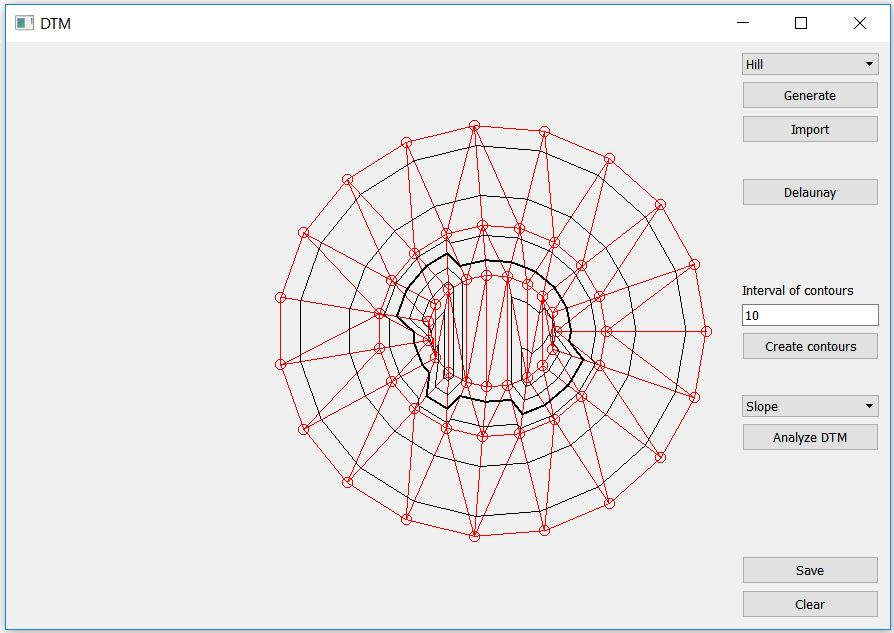
\includegraphics[width=7cm]{pictures/hill_bad.jpg}
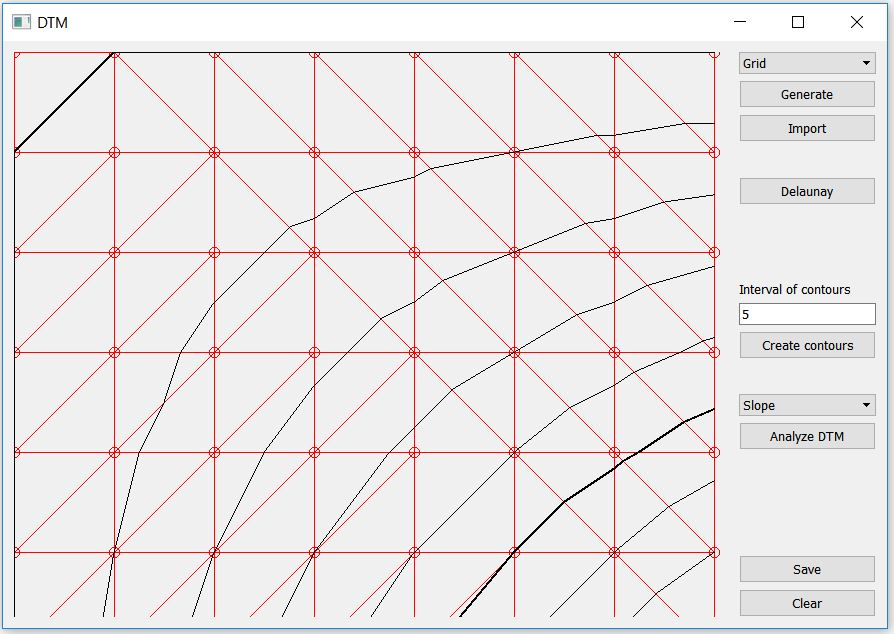
\includegraphics[width=7cm]{pictures/grid_ok.jpg}
\caption{Vrstevnice pro kupu vykresleny nekorektně, pro grid korektně}
\end{figure}

\subsection{Sklon a expozice terénu}
Při výpočtu sklonu a expozice terénu vzniká problém v rovinatém území. Při výpočtu vznikají zaokrouhlovací chyby, které se promítnou do sklonu a expozice. Proto se terén jeví uživateli nerovinný.\\
\\
Při vykreslení sklonu terénu byly pro ilustraci zvoleny odstíny šedi. Sklon nabývá hodnot od 0 do 180 $^\circ$. Vykreslení expozice bylo rozděleno do osmi směrů - S, SV, V, JV, J, JZ, Z, SZ. Barvy znázorňující jednolivé směry byly voleny asociativně s určitou symbolikou. Pro sever byla zvolena chladná modrá, pro jih naopak teplá červená barva. Pro východ byla zvolena žlutá barva reprezentující slunce a pro západ byla fialová, aby byla pokryta celá škála barev. Pro směry tvořené kombinací jiných směrů byla vybrána taková barva, pro kterou lze vidět určitý přechod obou barev. Pro kvalitnější znázornění expozice a jednotlivých přechodů by jistě bylo vhodnější použít více intervalů, neboť v prostředí Qt Creatoru můžeme vytvořit obrovské množství různých odstínů. Přesto by byl výsledek poté nepřehledný a uživatel by se v tom nemusel zcela orientovat. \\

\begin{figure}[h!]
\centering
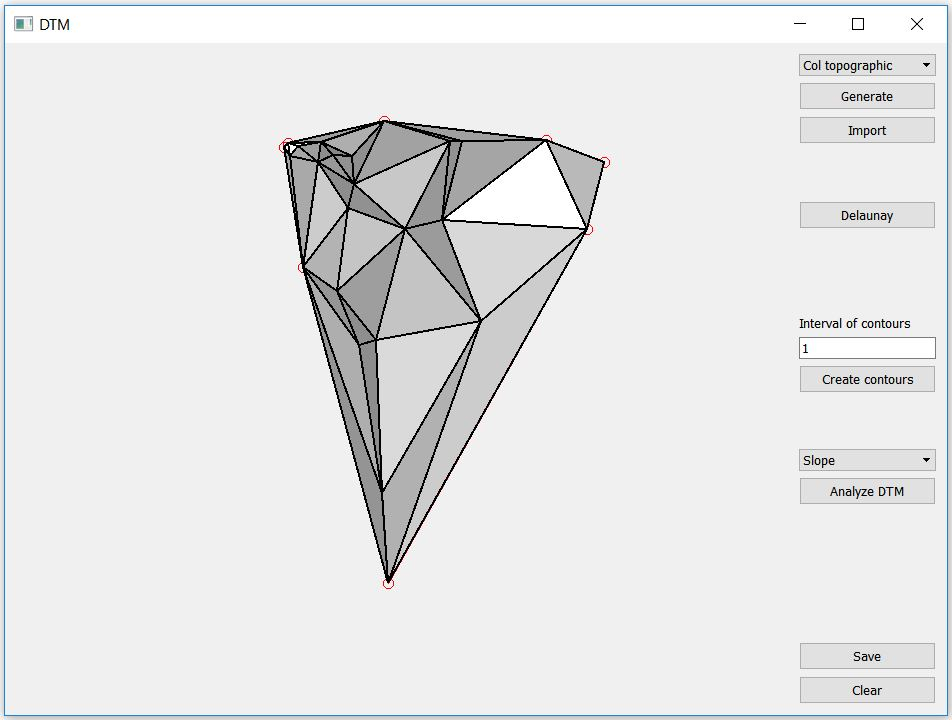
\includegraphics[width=7cm]{pictures/spocinek_sklon.jpg}
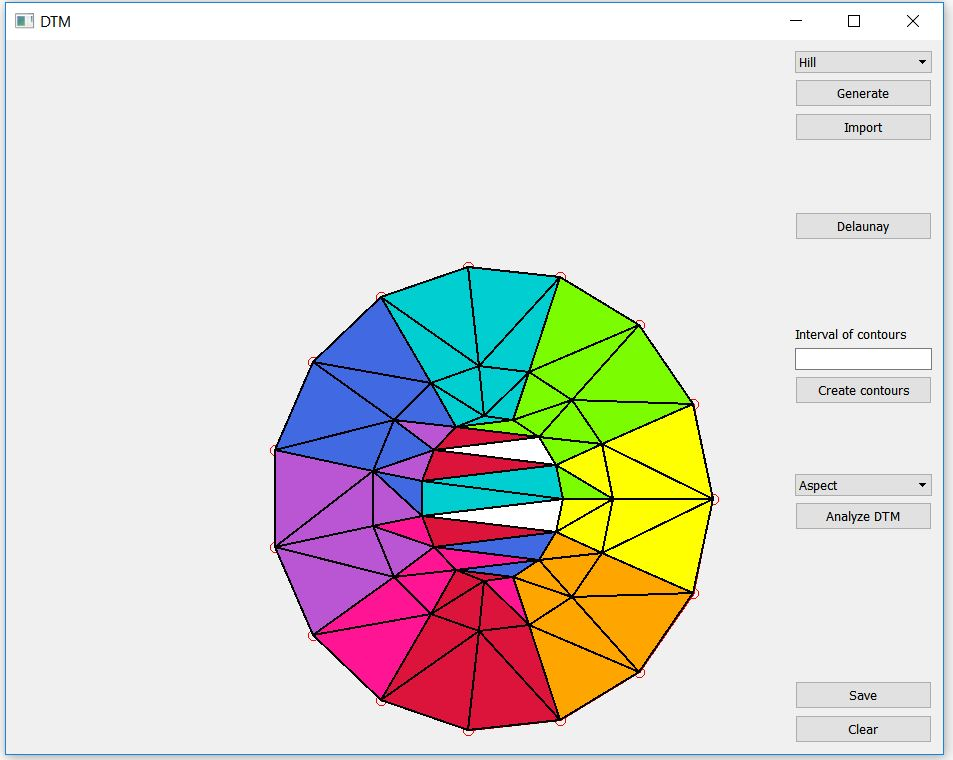
\includegraphics[width=7cm]{pictures/hill_aspect.jpg}
\caption{Sklon pro spočinek vykreslen korektně, expozice pro kupu téměř správě, až na oblasti, kde selhávaly i vrstevnice}
\end{figure}

Bylo by vhodné do aplikace umístit legendu expozice, neboť barvy samy o sobě uživateli nic neřeknou.

\subsection{Výstupy aplikace}
Uživatel má v aplikaci možnost uložit si vytvořený model naimportovaných souřadnic, Delaunay triangulací, vrstevnic, sklonu či expozice. Uživatel je vždy tázán na místo, kam nově vzniklý obrázek uložit. V případě úspěšného uložení je uživateli zobrazeno vyskakovací okno s informací o úspěšním uložení. \\

V rámci bonusových úloh byly také vytvořeny některé terénné útvary, například kupa, sedlo nebo údolí. Při tvorbě hřbetu došlo ke špatné implementaci a shodou náhod byl napsán takový kód, který vygeneruje spočinek. Generování spočinku je ovlivněno celou řadou proměnných, které jej generují. Záleží na zvoleném množství bodů, zadané generované vzdálenosti atd. Tato tvorba je také ovlivněna tím, že body se generují pouze v jednom kvadrantu, čímž se zvýší šance na to, aby byly poblíž sebe body se stejnou výškou a vytvořily tím spočinek. I přesto, že implementace spočinku je zcela náhodná, tudíž není korektní a občas se může stát, že spočinek nebude vygenerován, byla tato volba v kódu ponechána z toho důvodu, aby bylo možné na spočinku demonstrovat tvorbu vrstevnic a výpočet sklonu. \\ 

Co se týče výstupů aplikace, pro některé útvary funguje kód korektně, pro jiné se vyskytují chyby. Ukázky jednotlivých výsledků lze nalézt v kapitole 7 
- Aplikace. Níže následuje shrnutí jednotlivých metod a útvarů.\\

Při detailnějším zkoumání vrstevnic, pro údolí a hřbet jsou vrstevnice znázorněny korektně. Pro znázornění vrstevnic kupy však dochází k chybám a vrstevnice nejsou korektně zobrazeny. Důvodem je to, že body jsou na kružnici a Delaunay triangulace není vytvořena správně. Pro grid byly vrstevnice znázorněny také kvalitně, přestože je z obrázku vidět, že Delaunay triangulace není vytvořena zcela správně a při novém generování je triangulace sama o sobě nejednoznačná (v případě, že jako první testujeme náhodný bod). Vrstevnice pro spočinek jsou také chybně vykresleny, jedna ze zásad vrstevnic je to, že se jedná o uzavřenou linii, vrstevnice se navzájem nesmí křížit a nesmí se dvojit. Bohužel z výstupu aplikace je patrné, že tuto chybu program nedokáže eliminovat. Generování vrstevnic sedla je absolutně špatně. Vrstevnice se kříží, dvojí se, zobrazení sedla, kde by měla být ponechána mezera je vytvořena vrstevnice, která se na obou koncích duplikuje. Poměrně často je při generování sedla vytvořen i spočinek. \\

Pro sklon terénu je vyhodnocení také nejednoznačné. Pro hřbet i údolí je sklon vyobrazen korektně, neboť oblasti podél údolnice a hřbetnice mají shodnou výšku a oblasti směrem od hřbetnic/údolnic konstantně klesají/stoupají. Znázornění spočinku je také korektní, oblast je vykreslena bíle, tedy není zde žádný sklon, neboť oblast má konstantní výšku. Pro kupu je nekorektně vyobrazen střed, neboť v něm nejsou korektně vykresleny Delaunay trojúhelníky. \\

Vykreslení expozice je také nejednoznačné. Největší nedostatek je chybějící legenda, bez níž si uživatel není schopný představit, co která barva znamená. Pro zobrazení expozice kupy je pro vrchol opět špatně vypočtená. Ovšem pro následující místa je korektní a dle nastavených barev. Chybně je vyobrazena expozice i pro údolí a hřbet, kdy nastává stejný problém jako při gridu. Oblasti jsou vykresleny v závislosti na vytvořené triangulaci. Pro ukázku je vložena i expozice kresby gridu, která je silně závislá na vytvořené triangulaci. \\

Co se týče importovaných dat, textové soubory neobsahují výrazné terénní útvary, které by mohly ovlivnit výpočty. Navíc jsou podrobné body zaměřovány v okolí výrazných terénních útvarů ve větším množství. Vrstevnice, sklon i expozice byly pro importovaná data vykresleny korektně v rámci lineární interpolace. Pro kvalitnější výsledek by bylo vhodné použít nějakou funkci pro vyhlazení vrstevnic či pro tvorbu vrstevnic prostřednictvím morfologické interpolace.



\section{Náměty na vylepšení}
\subsection{Vrstevnice}
V aplikaci by bylo vhodné zobrazit popis jednotlivých vrstevnic dle kartografických zásad, aby měl uživatel jasnou představu o nadmořské výšce dané oblasti. Z důvodu čitelnosti byly totiž odstraněny popisy bodů obsahující nadmořskou výšku. Dále by stálo za zmínku přidat možnost pro nastavení výpočtu vrstevnic v nějakém rozsahu.\\

\subsection{Import dat}
V rámci aplikace by mohla být možnost volby odstranění bodů, nad kterými nechce uživatel počítat triangulaci. Při geodetickém zaměřování jsou výsledkem měření z totální stanice i orientační body, které se mohou nalézat ve výrazné vzdálenosti od zaměřovaných podrobných bodů a které značně znekvalitní vizualizaci. Pro použití této aplikace je tedy vhodné tyto body odstranit ručně.\\

\subsection{Sklon terénu}
Sklon terénu, jak je prostřednictvím aplikace vykreslován, vyvolává jen vizuální efekt. Uživatel si udělá přibližnou představu o terénu, ale tím to končí. Určitě by bylo vhodné sklonitost rozdělit do intervalů. V případě, že by aplikace měla praktické využití, kdy by jí například využívali stavaři, kteří při výkopu musí zkontrolovat sklon vzhledem k druhu horniny a přípustnému sklonu svahu, by bylo rozdělení barev dle intervalů určitě vhodné.\\

\subsection{Tlačítka aplikace}
Jedním z možných vylepšení aplikace je určitě nastavení dostupnosti tlačítek (Unabled, Disabled). V aplikaci je prozatím vyřešen jen neplatný vstup intervalu vrstevnic.\\


\clearpage
\section{Reference}

\begin{enumerate}
\item  BAYER, Tomáš. Geometrické vyhledávání [online][cit. 1. 12.2018]. \\
Dostupné z: https://web.natur.cuni.cz/~bayertom/images/courses/Adk/adk5.pdf  \\

\item JANEČKA, Karel, PACINA, Jan. Výukové materiály k předmětu KMA/UGI - Západočeská univerzita v Plzni. [online][cit. 4. 12. 2018]\\
Dostupné z: https://kgm.zcu.cz/studium/ugi/cviceni/ch08s01.html\\

\item BENEŠ, Petr. Diplomová práce: Voroného diagramy v molekulární chemii. [online] [cit. 4. 12. 2018]\\
Dostupné z: https://is.muni.cz/th/m1tcs/benes\_dp.pdf \\

\item PUCKEY, Jonathan. Delaunay Raster. [online] [cit. 4. 12. 2018]\\
Dostupné z: https://jonathanpuckey.com/projects/delaunay-raster/index.html

\item VÚGTK. Terminologický slovník zeměměřictví a katastru nemovitostí. [online] [cit. 5. 12. 2018]\\
Dostupné z: https://www.vugtk.cz/slovnik/index.php \\



\end{enumerate}
\end{document}



 